\documentclass[11pt,a4paper,titlepage]{article}
\usepackage{mypackages}

%title information
\title{Paper Title v3}
\author{Your Name}



\begin{document}

\maketitle

\pagenumbering{roman}

\clearpage

\tableofcontents

\clearpage

\pagenumbering{arabic}

\section{Introduction}
\section{Research}
\section{Analysis}
\section{Discussion}
\section{Evaluation}

\section{\LaTeX{} help}

\subsection{General Help}

\url{https://www.sharelatex.com/learn/}


\subsection{Equations}

From Equation \eqref{eq:einsteinequation} \ldots


\begin{equation}
\label{eq:einsteinequation}
E = m c^2
\end{equation}

Here is a not numbered equation:

\begin{equation*}
\label{eq:einsteinequation*}
E = m c^2
\end{equation*}


Here is an aligned equation:
\begin{align}
(a+b)^2  & = (a+b)(a+b)  \nonumber \\
  & = a^2+2ab+b^2 \label{eq:aplusbexpanded}
\end{align}


Math can also be writing in line $1-\frac{1}{3}+\frac{1}{5}-\frac{1}{7}+\frac{1}{9}-\ldots = \frac{\pi}{4}$

\subsection{Lists}

\begin{enumerate}
\item cake
\item cookies
\end{enumerate}

\dots or bullet points \dots

\begin{itemize}
\item cake
\item cookies
\end{itemize}


\subsection{Figures}
The figures environment provides an environment that allows figures to be properly formatted.
\subsubsection{Images}

Images are included by using the graphicx environment by using the \texttt{figure} environment and the \texttt{includegraphics} command. An example of an image being inserted can be seen in \ref{fig:einstein}, it was done as follows:

\begin{lstlisting}[breaklines]
\begin{figure}[h]
\centering
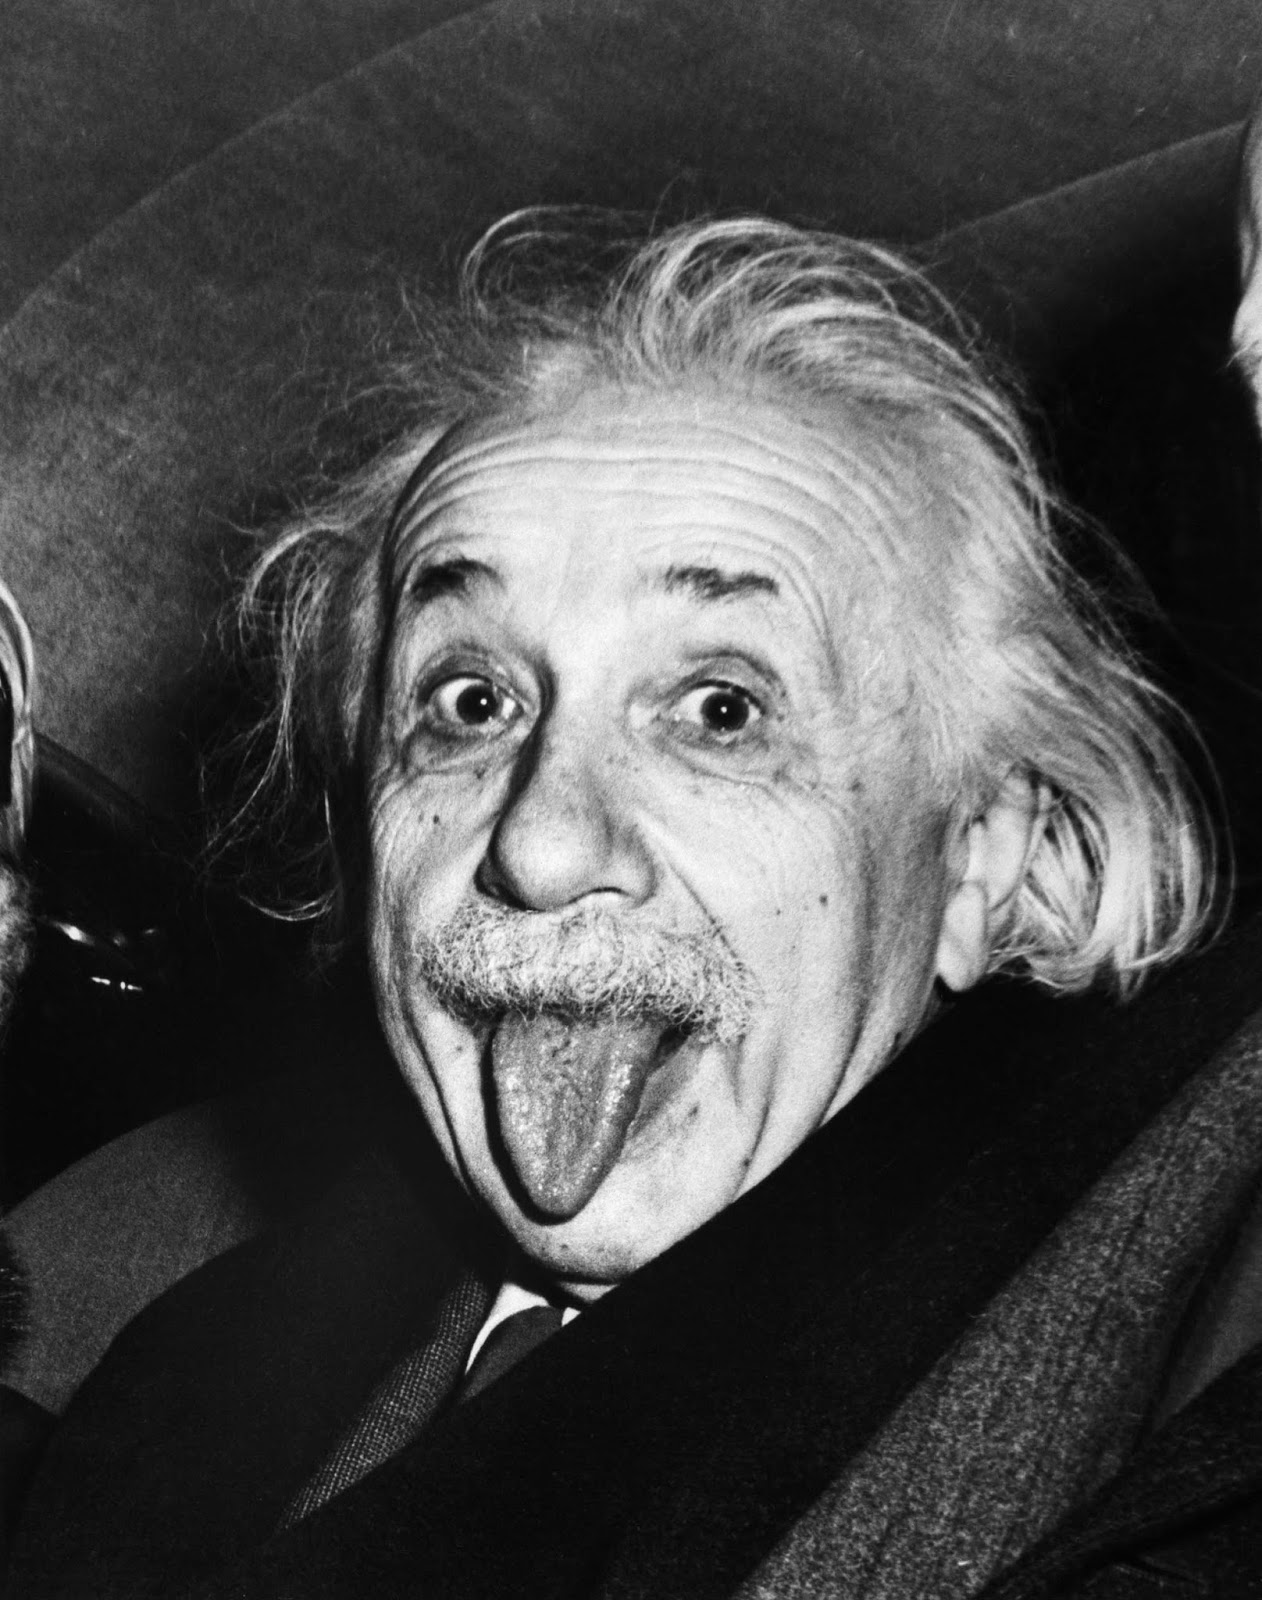
\includegraphics[width=0.3\textwidth]{einstein.jpg}
\caption{\label{fig:einstein} Albert Einstein on his 72nd Birthday (14 March 1951) \cite{ArthurSasse}.}
\end{figure}
\end{lstlisting}

\begin{figure}[h]
\centering
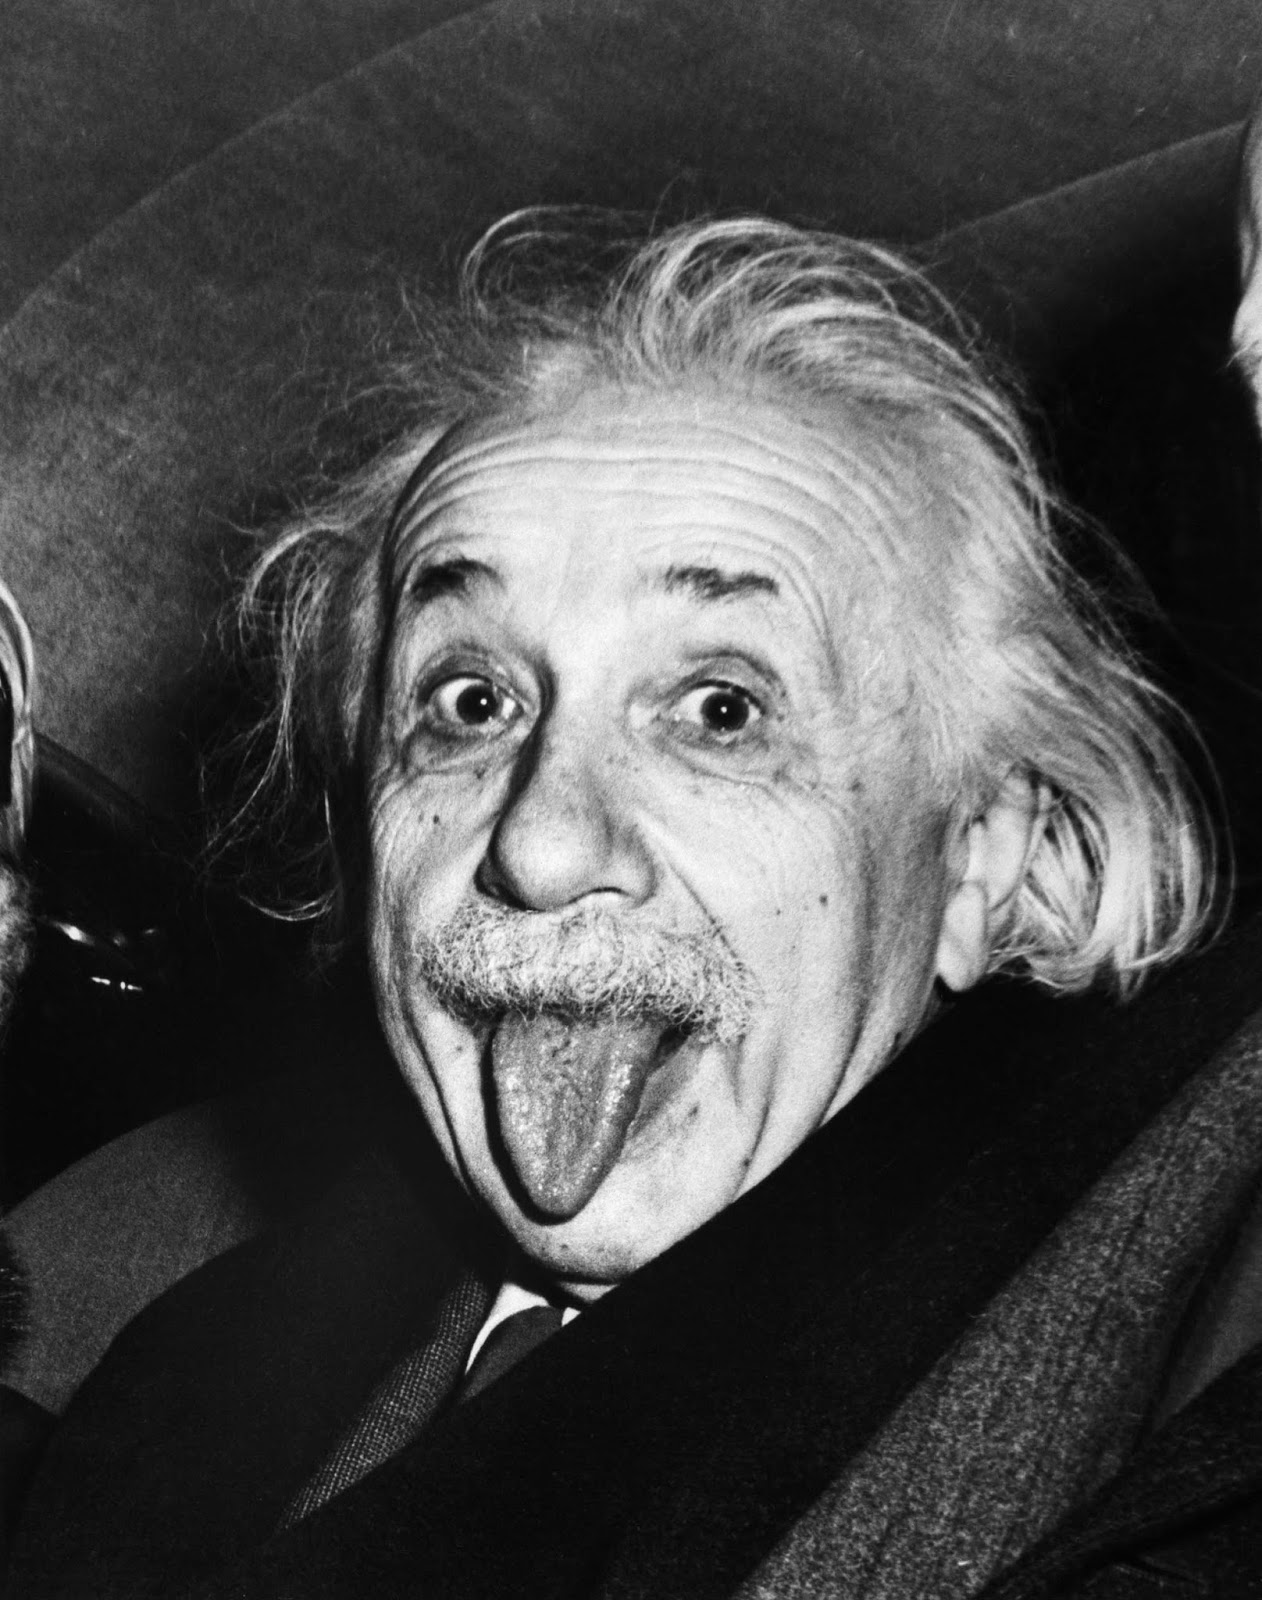
\includegraphics[width=0.3\textwidth]{einstein.jpg}
\caption{\label{fig:einstein} Albert Einstein on his 72nd Birthday (14 March 1951) \cite{ArthurSasse}.}
\end{figure}

\subsubsection{TikZ Drawing}
You can also draw directly in \LaTeX{} using the TikZ package, however you draw by defining the shapes through using a coordinate system.


\begin{figure}[h]
\centering


\begin{tikzpicture}
\draw[ultra thick] (0,0) -- (5,0);
\draw[ultra thick] (0,0) -- (0,0.5);
\draw[ultra thick] (5,0) -- (5,0.5);
\draw[ultra thick] (0,0.5) -- (2.25,0.5);
\draw[ultra thick] (5,0.5) -- (2.75,0.5);
\draw[ultra thick] (2.25,0.5) -- (2.25,5.5);
\draw[ultra thick] (2.75,0.5) -- (2.75,5.5);
\draw[ultra thick] (2.25,5.5) -- (0,5.5);
\draw[ultra thick] (2.75,5.5) -- (5,5.5);
\draw[ultra thick] (0,5.5) -- (0,6);
\draw[ultra thick] (5,5.5) -- (5,6);
\draw[ultra thick] (0,6) -- (5,6);
 
\end{tikzpicture}
\caption{I Beam cross-section}
\label{fig:I_beam}
\end{figure}


I typically put the tikzpicture in a figure environment, as seen in Figure \ref{fig:I_beam}.

See \href{http://texample.net/TikZ/}{this} for some TikZ examples.
\subsubsection{Figure Position}


\subsection{Table}

% Note this table uses the booktabs package
\begin{table}[h]
\centering
\caption{Booktabs table}
\label{tbl:table1}
\begin{tabular}{@{}lll@{}}
\toprule
Text1    & Text2      & Text3 \\ \midrule
1        & 3          & 2     \\
How come & \textbf{4} & Hello \\ \bottomrule
\end{tabular}
\end{table}


Tables in \LaTeX{} % the {} is for space
are not the most convenient, as seen by Table \ref{tbl:table1} verbatim:

\begin{verbatim}
\begin{table}[h]
\centering
\caption{Booktabs table}
\label{tbl:table1}
\begin{tabular}{@{}lll@{}}
\toprule
Text1    & Text2      & Text3 \\ \midrule
1        & 3          & 2     \\
How come & \textbf{4} & Hello \\ \bottomrule
\end{tabular}
\end{table}
\end{verbatim}

Therefore I strongly using an online table generator such as \href{https://www.tablesgenerator.com/latex_tables}{tablesgenerator.com}, as this can get much more complex. Moreover you can load tables in from excel.

\medskip

\subsection{Verbatim Environments}

\texttt{verbatim} environments are used to display computer text, in larger environment as opposed to using \texttt{\textbackslash texttt\{\}}. It work well for pseudocode too. However, generally it is recommended to use the \texttt{listings} environment giving its plethora of features. 

\begin{verbatim}
xtick = [j*100 for j in range(11)]
ytick = [k*10 for k in range(11)]
\end{verbatim}

\subsection{Code listings}

However, for listing code, another environment exist (\texttt{listings}) that is more well adapt, by allowing syntax highlighting among other features.

\begin{lstlisting}[language=Python]
W=[] #winnning positions
L=[0] #//losing positions
D=[] #// Difference between losing positions
a = input("Enter first number of coins which can be removed: ")
b = input("Enter second number of coins which can be removed: ")
c = input("Enter third number of coins which can be removed: ")
x = input("Enter total number of coins that are in the pile: ")

for i in range (1,int(x)):
  if ((i-int(a)) in L or (i-int(b)) in L or (i-int(c)) in L) :
      W.append(i)
  else:
        L.append(i)
for e in range (1,len(L)):
    D.append(L[e]-L[e-1])


print("Information for",a,b,c)
print ("-"*80)
print("Win:", W)
print("Lose:", L)
print("Difference between Losing positions:", D)
\end{lstlisting}


\subsection{Referencing in \LaTeX{}}

Referencing in \LaTeX{} is nice and annoying at the same time. You have to write out the content attributes, however it does in text referencing for you by using  the cite command with the reference key in the curly bracket. Note that there are different bibliography styles so make sure to change it to the one your school/uni is using. You can do this by simply searching.

\url{https://www.sharelatex.com/learn/Bibtex_bibliography_styles}



\bibliographystyle{agsm} % you should change the style
\bibliography{references}


\clearpage
\appendix


\section{Appendix Item 1}
\label{appendix:Appendix1}

\section{Appendix Item 2}
\label{appendix:Appendix2}

\end{document}
